\documentclass{beamer}

\usetheme{Madrid}

\usepackage{graphicx}
\usepackage{amsmath,amssymb}
\usepackage{caption}

\DeclareMathOperator{\E}{\mathbb{E}}
\captionsetup[figure]{labelformat=empty}

\title[]{The Impact of Imputation Quality on Family Based Analysis}
\author[]{Mahdi Mir}
\institute[]{SSGAC}
\date[]{Oct 2024}

\begin{document}

\maketitle

\begin{frame}{What is imputation?}
      \begin{itemize}
            % First, I give a brief introduction to imputation.
            \item Imputation is a process in which we predict the genotypes that are not directly observed.
            % Explain that not all genotypes can be measured directly due to limitations in technology or resources.
            % We use the information from the observed genotypes to predict the unobserved genotypes.
            % Here, we leverage existing data to fill in the gaps.
            % also we use a reference panel to predict the genotypes that are not directly observed.
            \item We use the information from the observed genotypes and a reference panel to predict the unobserved genotypes.
      \end{itemize}
\end{frame}

\begin{frame}{What is imputation?}
      % this figure from Zheng et al. (2011) is a good visual representation of the imputation process.
      % suppose we a have reference panel and we have some genotypes that are directly observed.
      % and also we have some genotypes that are not directly observed.
      % in the imputation process we are going to use the information from the reference panel and the observed genotypes to predict the unobserved genotypes.
      % the predicted genotypes are called imputed genotypes.
      % for the genotyps that we don't know we can have best guess for them or we can have a range of possible genotypes.
      % we can have a probability distribution for the genotypes that we don't know.
      \begin{figure}
            \centering
            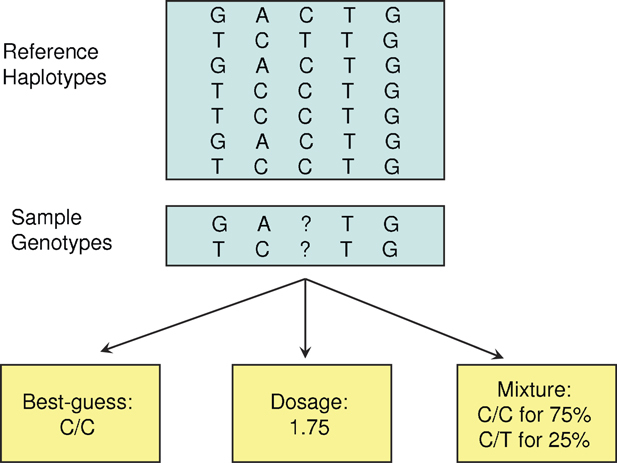
\includegraphics[width= .7\textwidth]{fig/mfig001-2.jpg}
            \caption{Source: Zheng et al. (2011)}
      \end{figure}
\end{frame}

\begin{frame}{Why Imputation?}
      \begin{itemize}
            \item Imputation is used to increase the number of SNPs that are available for analysis.
            % This allows us to have more data points for our studies, leading to potentially stronger conclusions.
            \item Imputation is used in GWAS to increase the power of the study.
            % Highlight how this contributes to the overall strength of genetic studies.
      \end{itemize}
\end{frame}

\begin{frame}{Motivation}
      \begin{itemize}
            \item We are concerned that low-quality imputed genotypes may not work for family-based analysis. % and maybe for other types of analysis
            \item We are interested in understanding the impact of imputation quality on downstream analysis.
            % Point out the risk of relying on low-quality data.
            \item Family-based research designs rely on special properties of family data that might not be preserved in low-quality imputed genotypes.
            % Explain the importance of quality in family-based studies.
            \item E.g.: In theory by the Mendelian laws we expect the correlation between sibling pairs and parent-offspring pairs genotypes to be 0.5.
            % Reinforce the idea that expectations are based on genetic principles.
            \item Current imputation methods do not take into account the relationships between the individuals.
      \end{itemize}
\end{frame}

\begin{frame}{Introduction}
      \begin{itemize}
            % Now I am going to outline what we will discuss in this presentation.
            \item We are going to show some correlation analysis between sibling pairs and parent-offspring pairs.
            % Briefly explain the significance of these correlations.
            \item We show the low-quality imputed genotypes correlation deviates from the theoretical expectations.
            % This is crucial as it raises questions about the validity of low-quality imputation.
            \item E.g.: Howe et.al (2022) Sib-GWAS paper used low-quality imputed SNPs in its analysis.
            % Mention this as an example of a potential pitfall in research.
      \end{itemize}
\end{frame}

\begin{frame}{Correlation Analysis on the Imputed Data}
      \begin{itemize}
          \item In theory, we should see 0.5 correlation between both full-sibling and parent-offspring pairs genotypes.
          % Explain the theoretical background for this expectation.
          \item So if the imputed genotypes are of high quality, then we should see the distribution of correlations to be concentrated around the half.
          % Stress the importance of quality in ensuring expected results.
          \item Expectation: we would expect more deviation for low-quality SNPs from the theoretical expectation.
          % Set the stage for the data and findings that will follow.
      \end{itemize}
\end{frame}

% In this part, we have some figures that effectively convey our point.
% Each step of the analysis has its own challenges, but we won't go into too much technical detail here.

\begin{frame}{Sample}
      \begin{itemize}
            \item UKB Imputed Data.
            % Mention the relevance of the UK Biobank in this context.
            \item \(19K\) sibling pairs.
            % Emphasize the size of the dataset as a strength.
            \item \(4K\) parent-offspring pairs.
            % Highlight the significance of this data for the analysis.
      \end{itemize}
\end{frame}

\begin{frame}{Correlations Distribution - Full Siblings}
      \begin{columns}
            \begin{column}{0.5\textwidth}
                  \centering
                  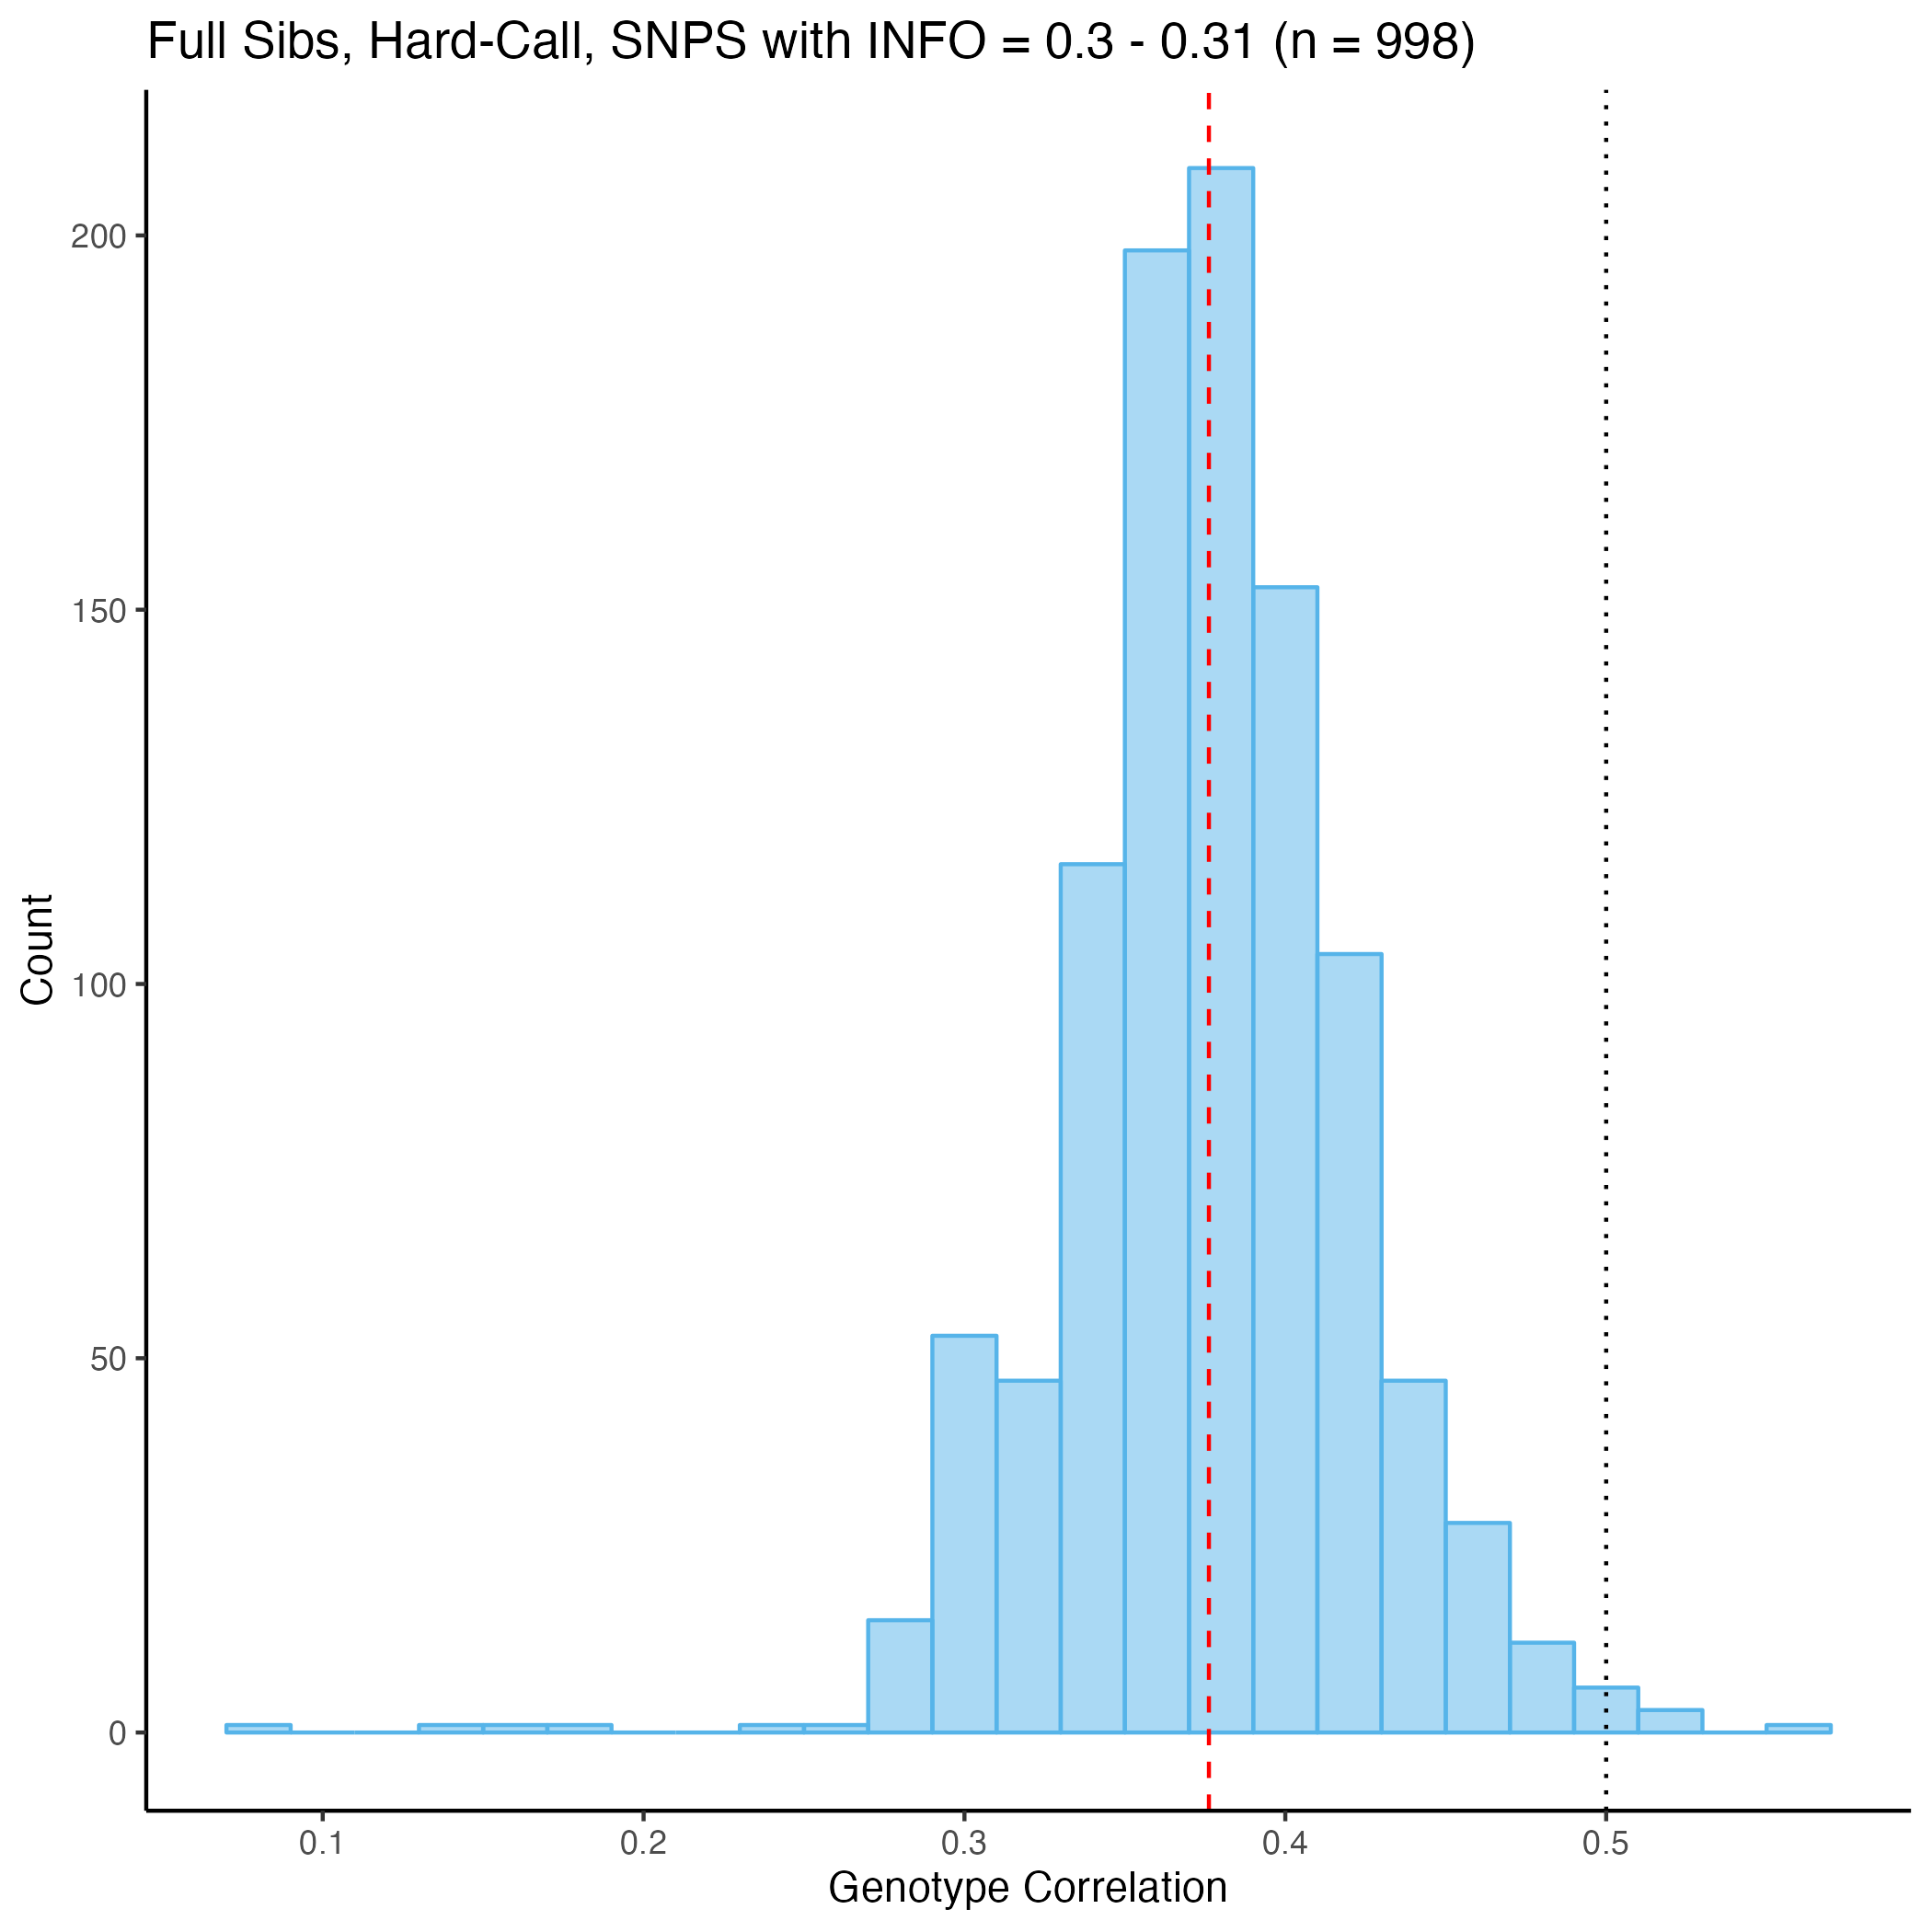
\includegraphics[width= \textwidth]{fig/FS-HC-i30.png}
                  \captionof{figure}{Low Quality Imputed SNPs}
              \end{column}
            \begin{column}{0.5\textwidth}
                \centering
                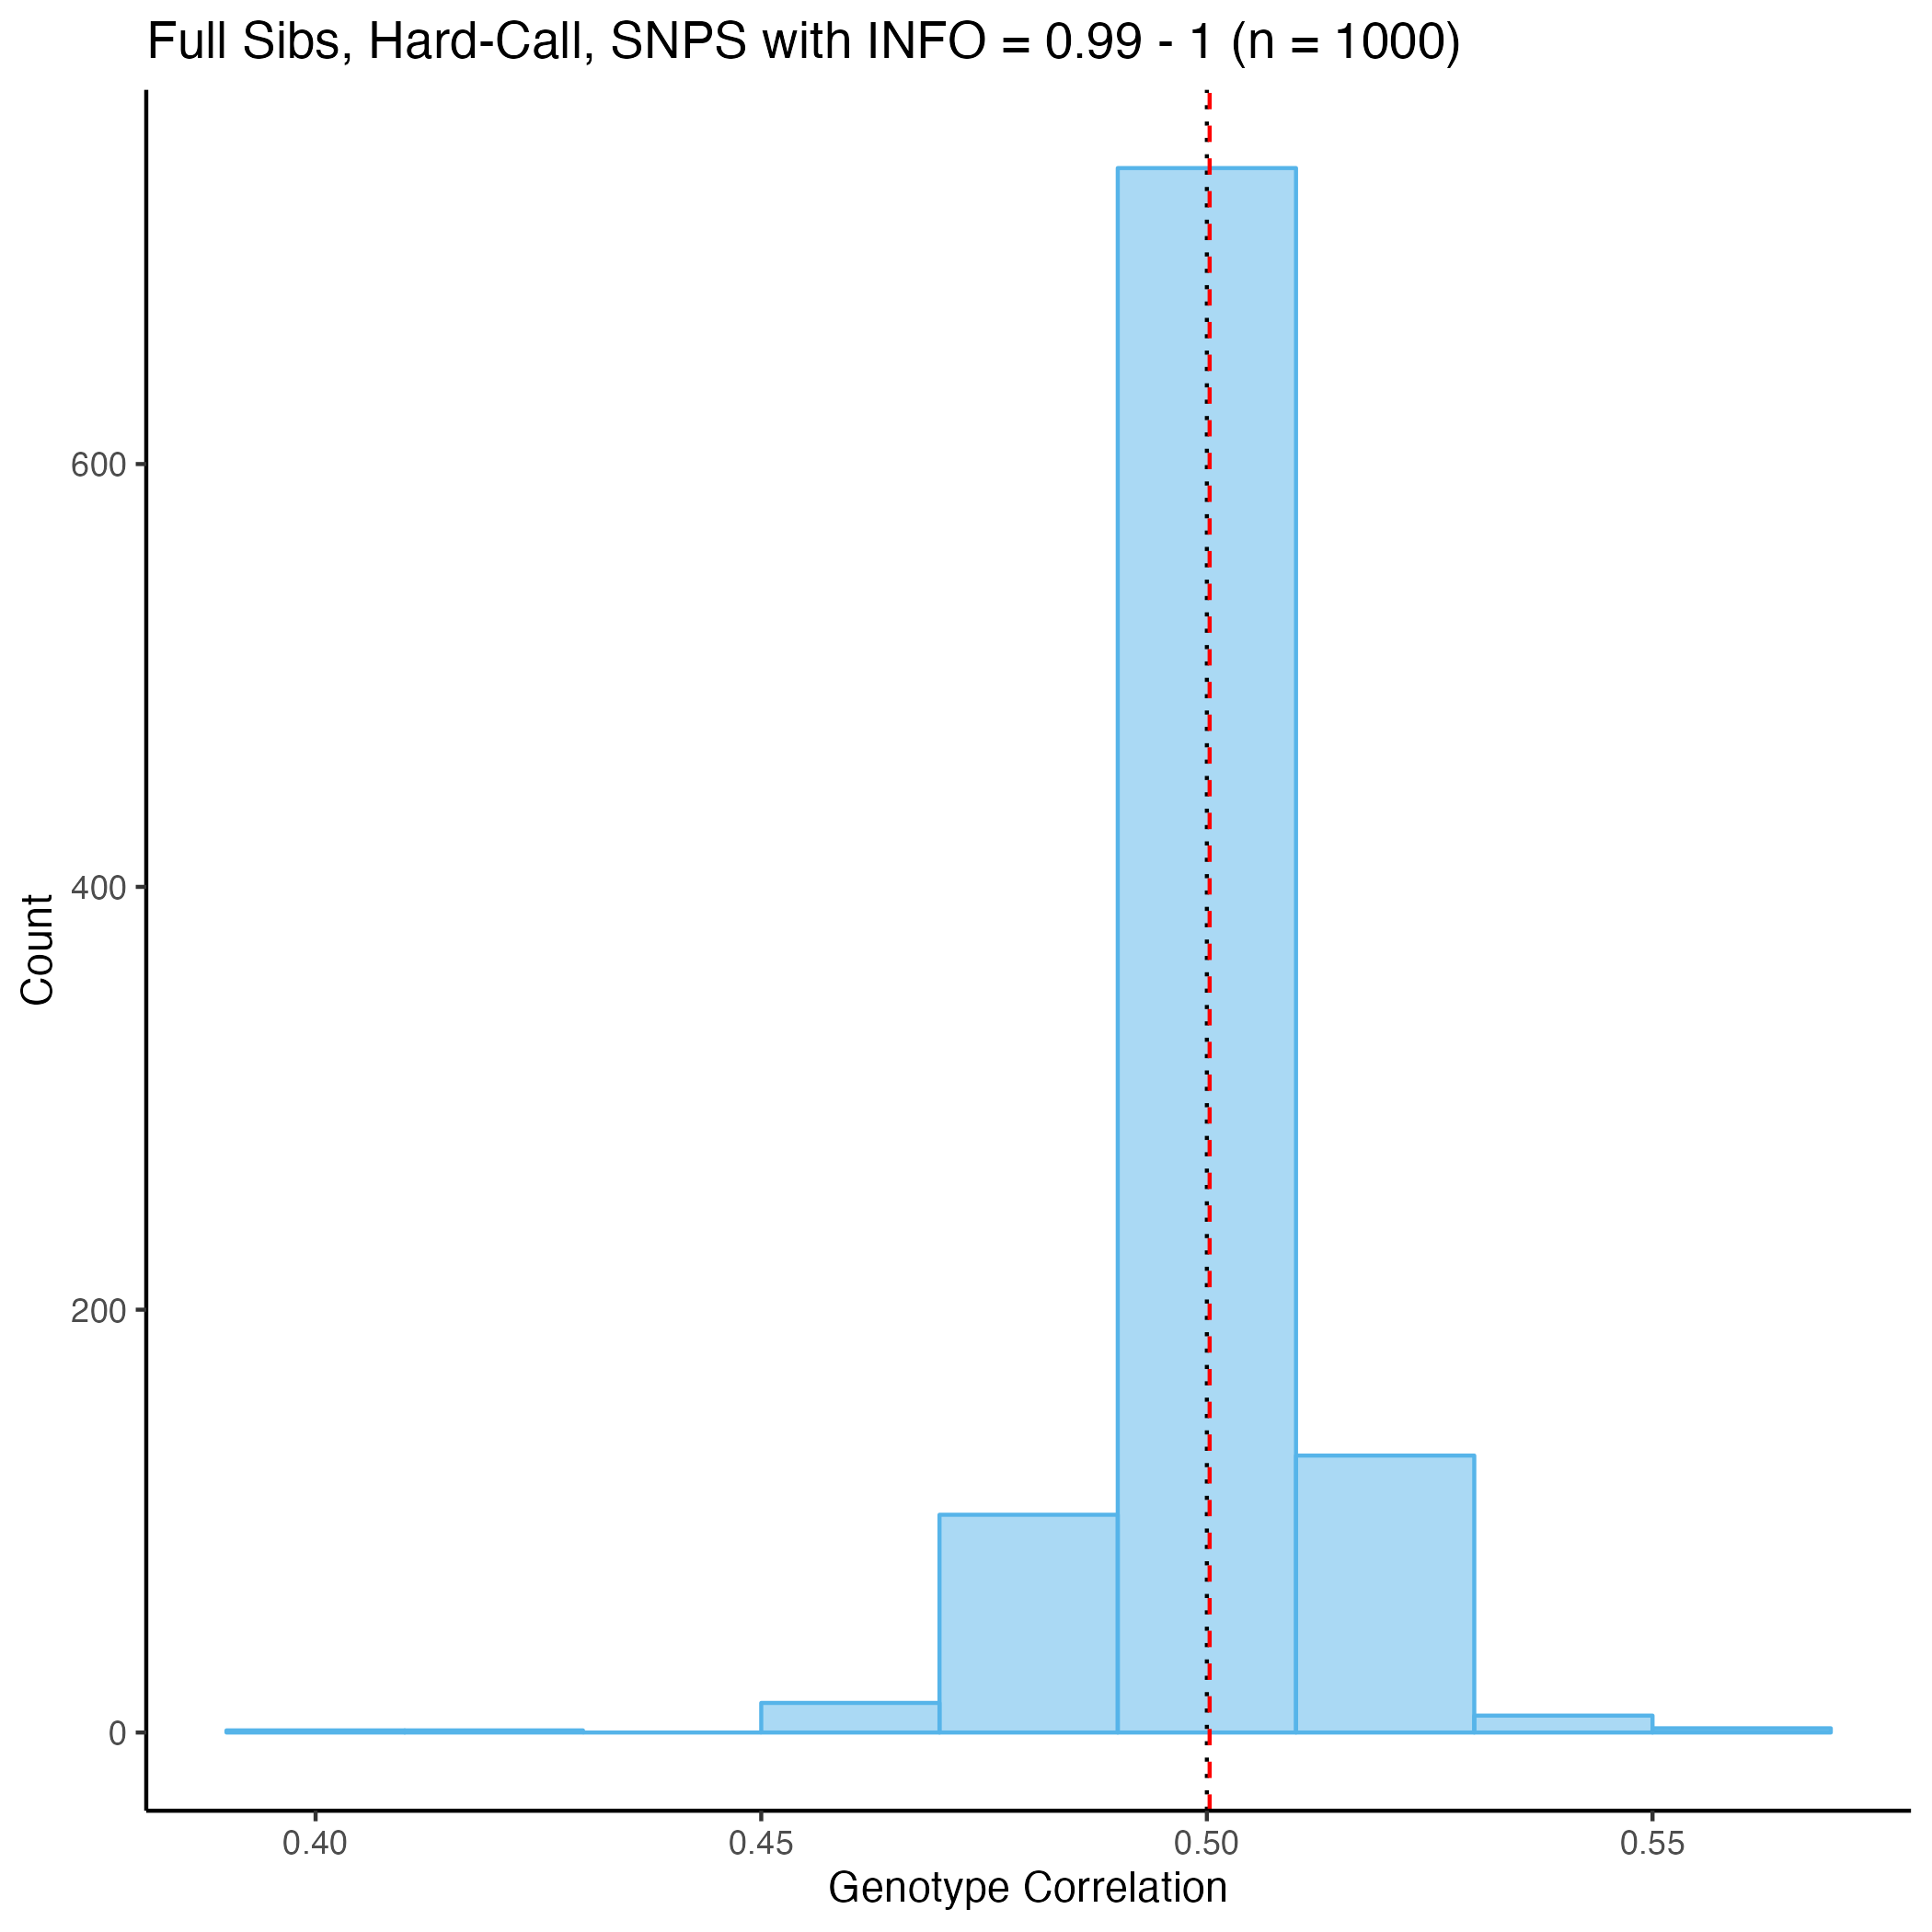
\includegraphics[width= \textwidth]{fig/FS-HC-i99.png}
                \captionof{figure}{High Quality Imputed SNPs}
            \end{column}
        \end{columns}       
      % Discuss the difference in distributions here, indicating the impact of imputation quality.
\end{frame}

\begin{frame}{Correlations Distribution - Parent-Offspring}
      \begin{columns}
            \begin{column}{0.5\textwidth}
                  \centering
                  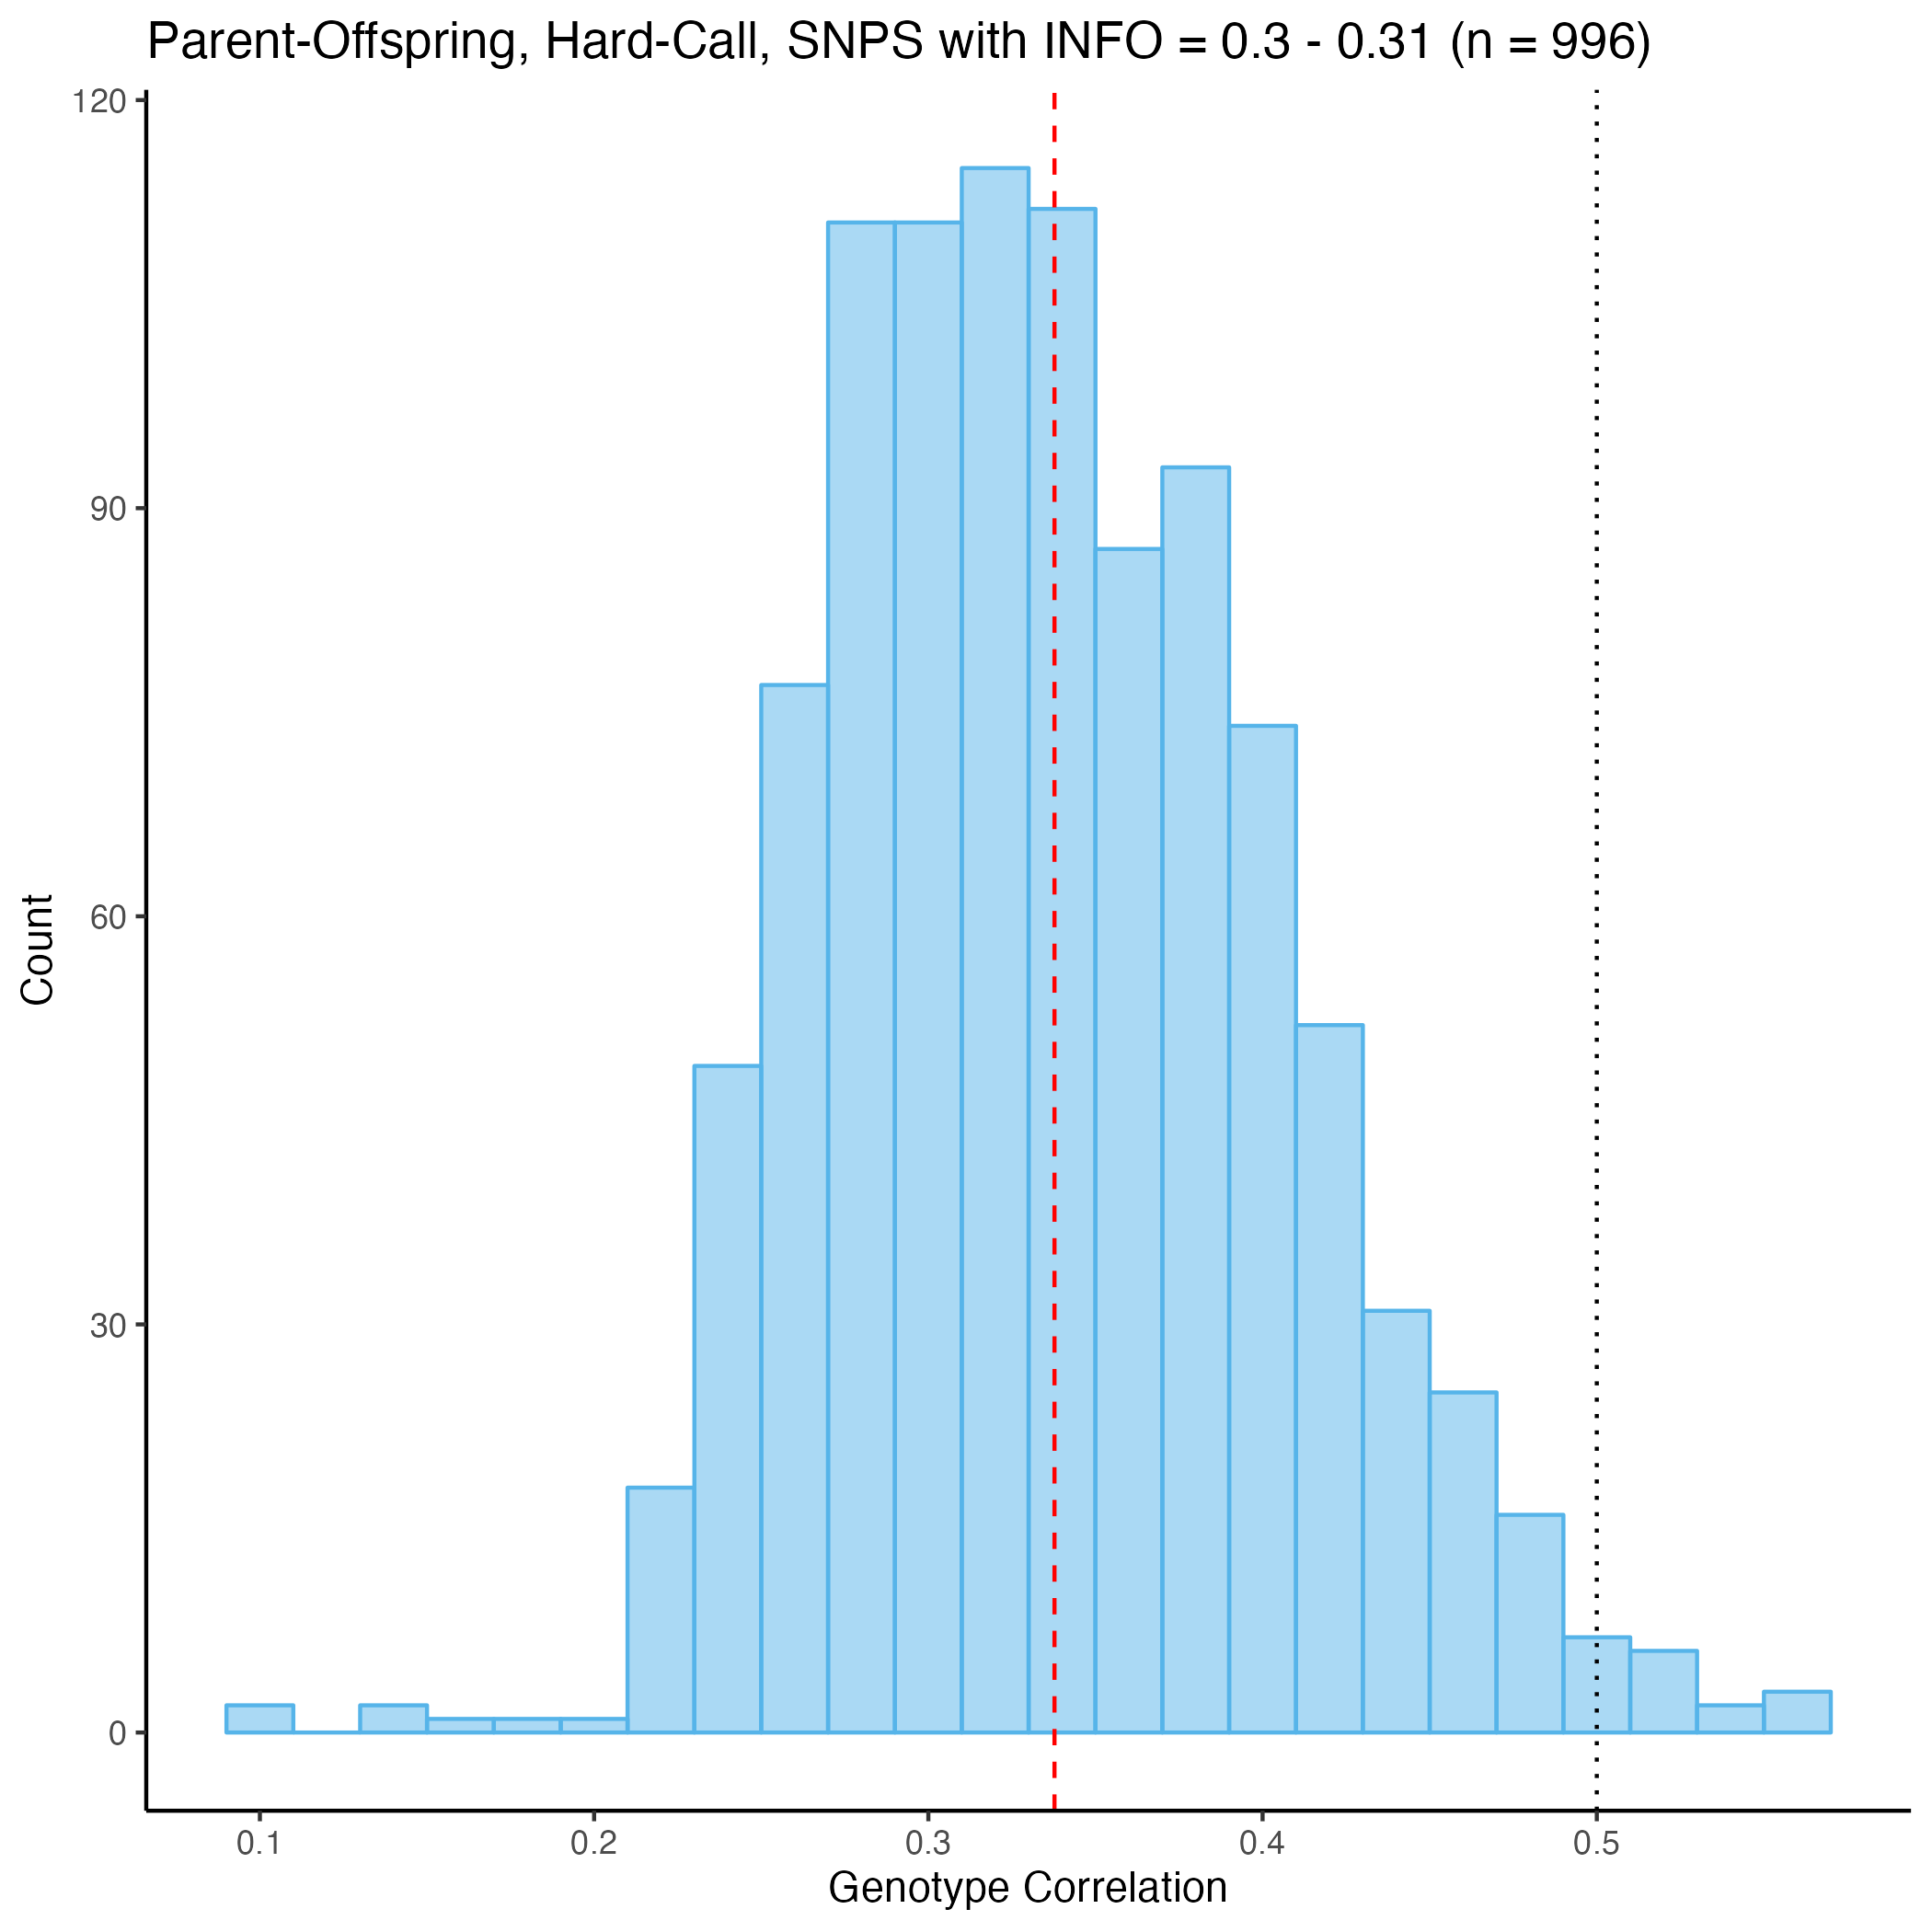
\includegraphics[width= \textwidth]{fig/PO-HC-i30.png}
                  \captionof{figure}{Low Quality Imputed SNPs}
              \end{column}
            \begin{column}{0.5\textwidth}
                \centering
                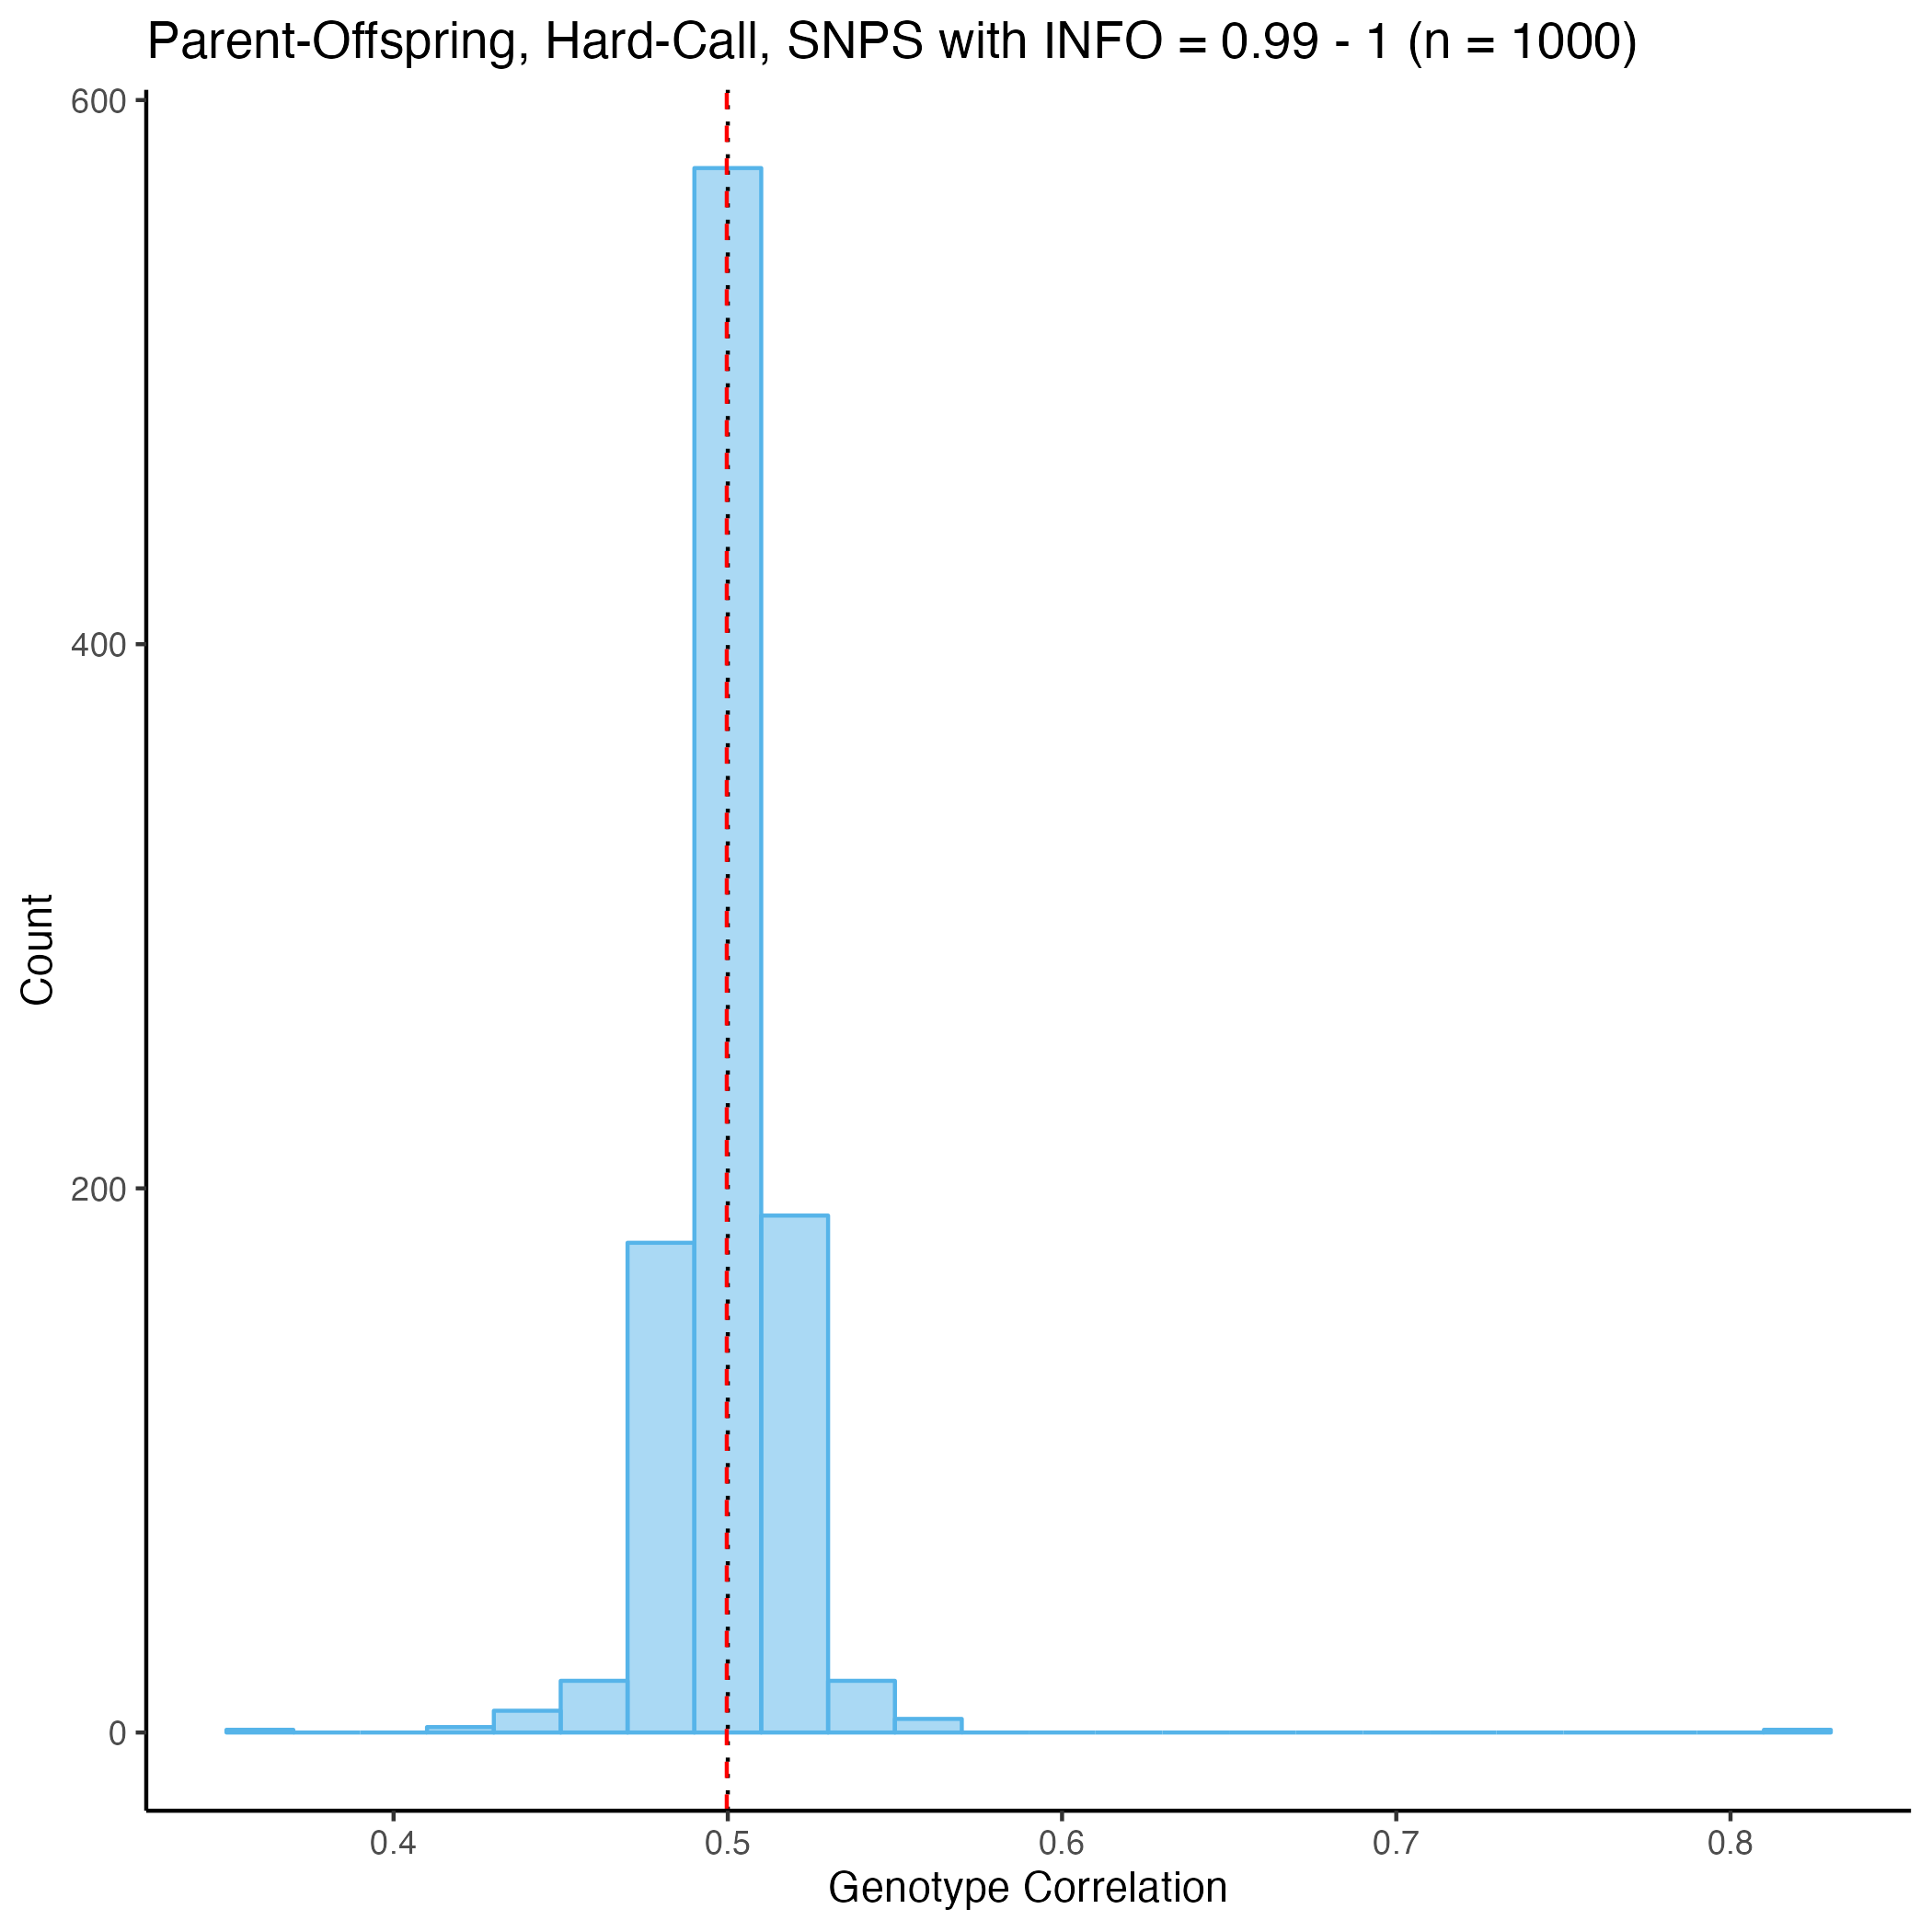
\includegraphics[width= \textwidth]{fig/PO-HC-i99.png}
                \captionof{figure}{High Quality Imputed SNPs}
            \end{column}
        \end{columns}       
      % Similarly, analyze the parent-offspring correlations and their implications.
\end{frame}

\begin{frame}{Mean Genotype Correlation}
      \centering
      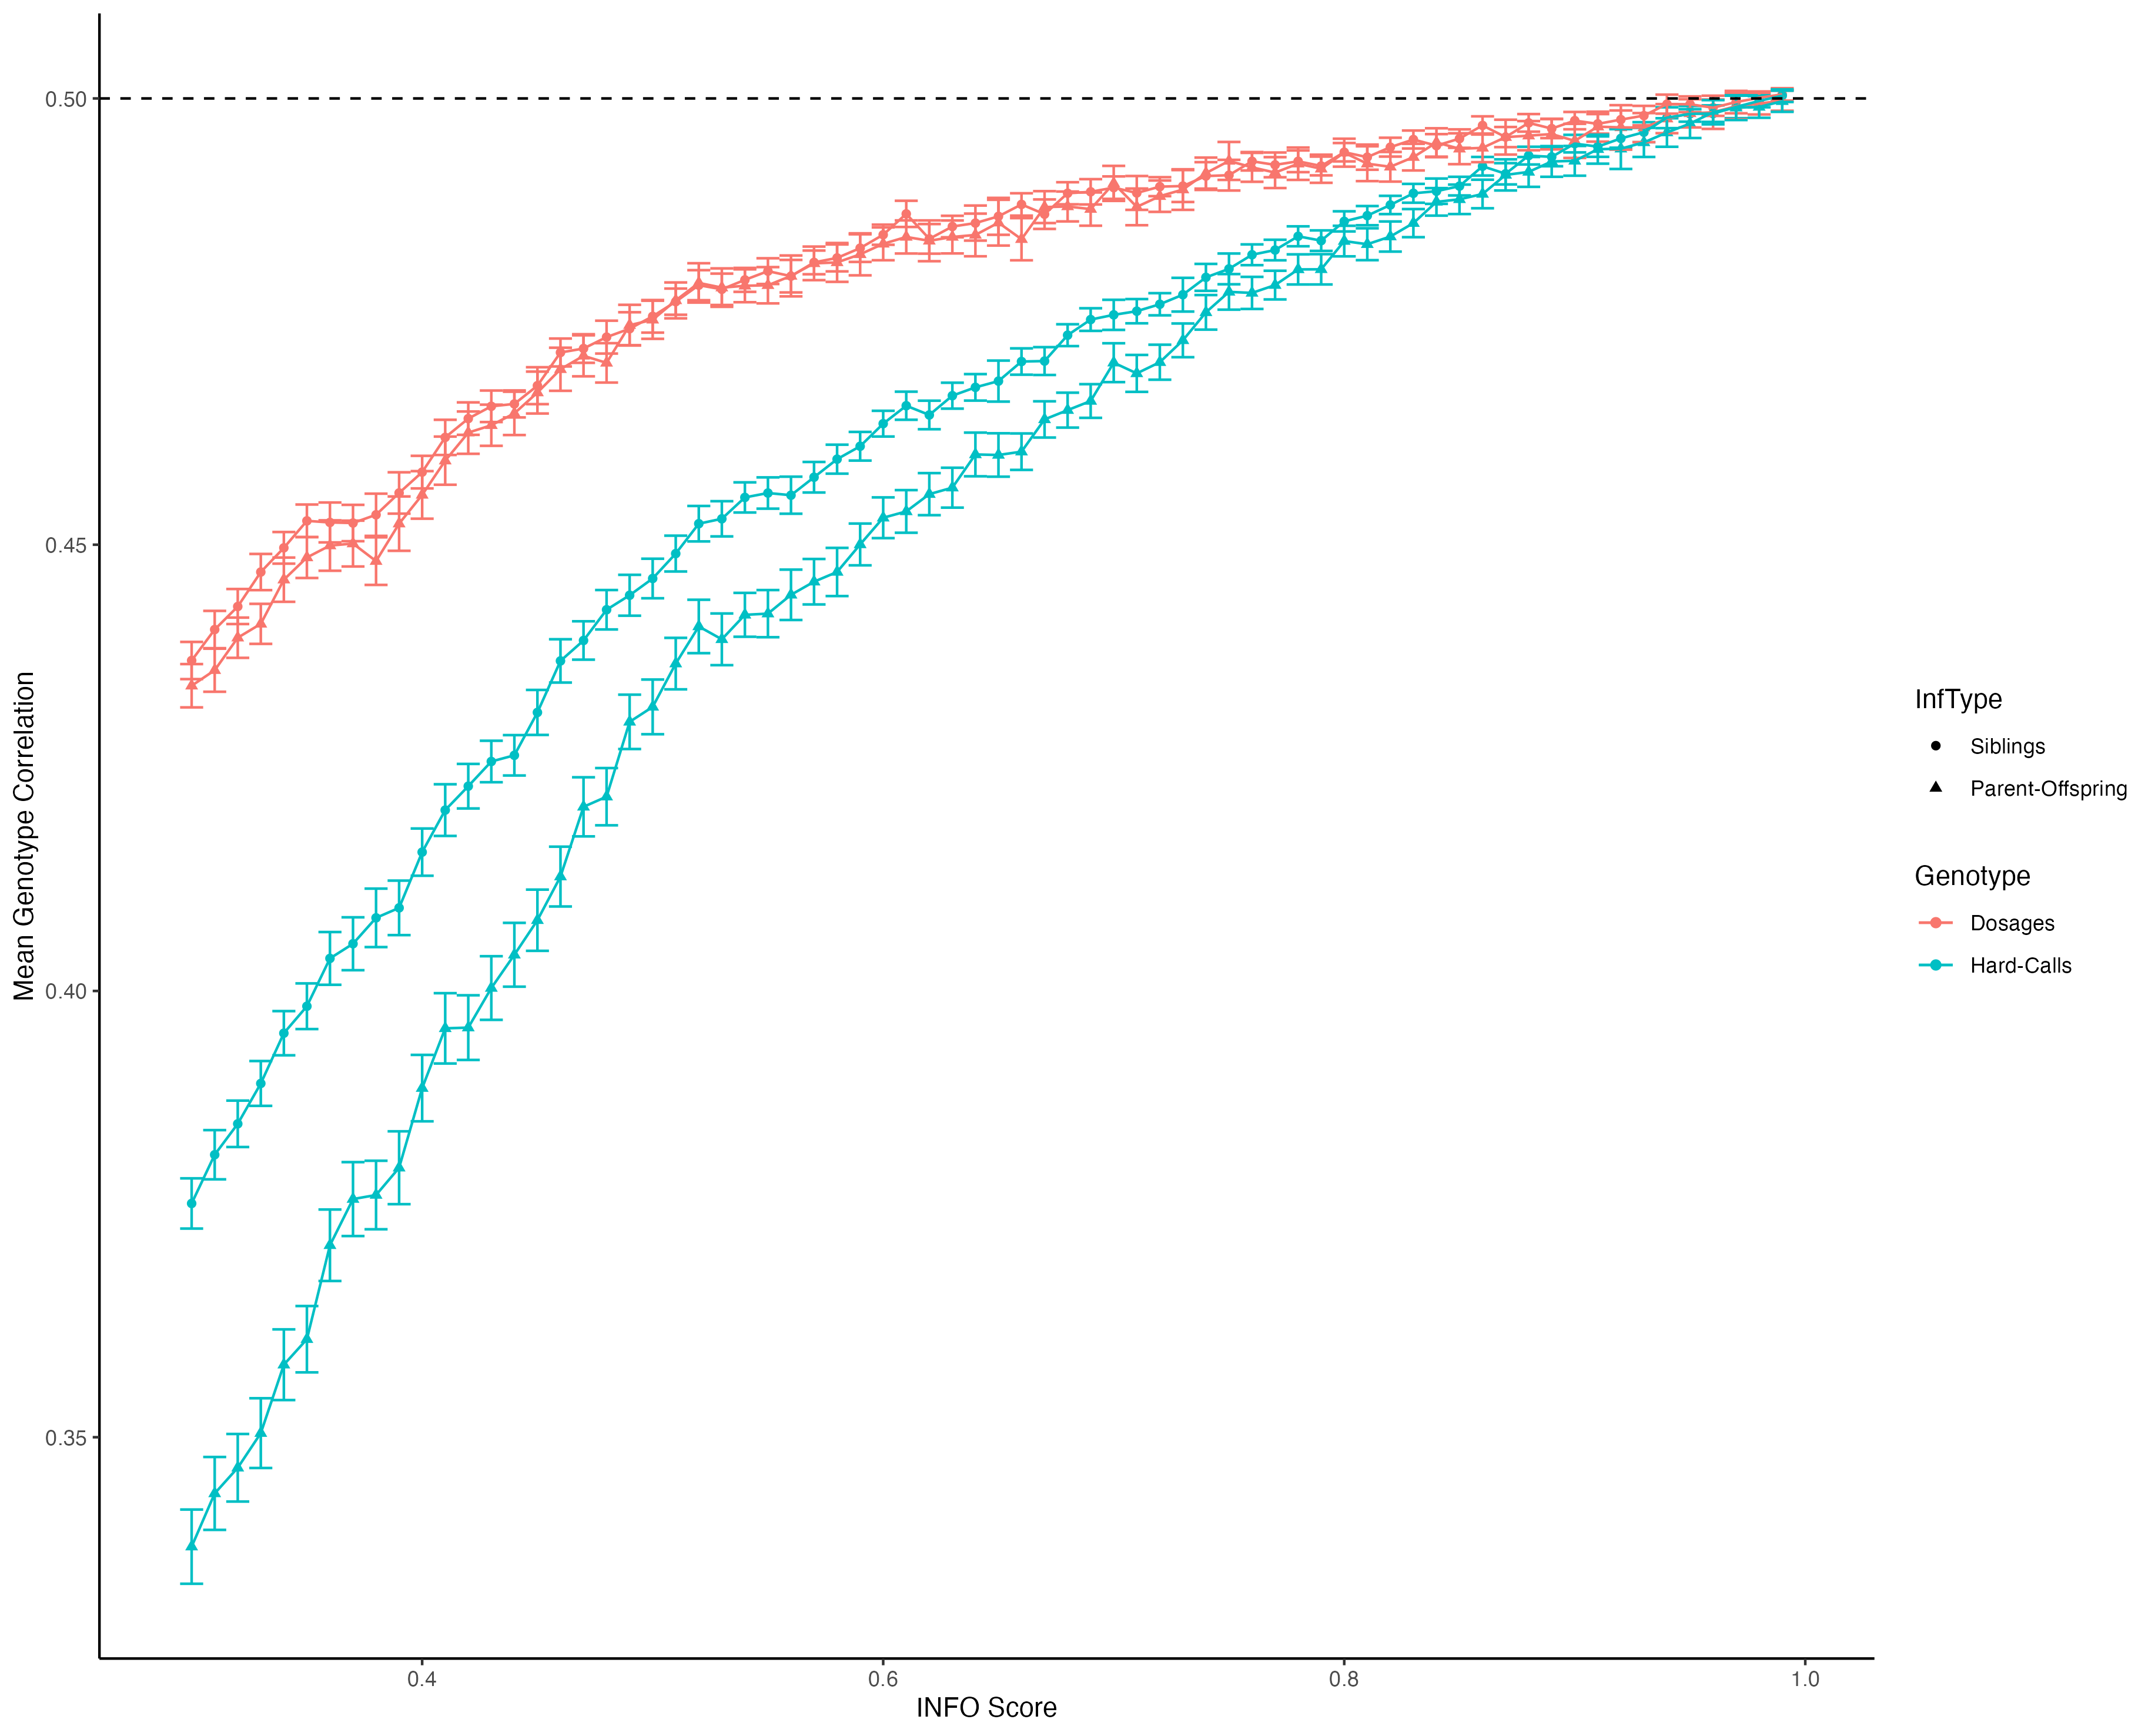
\includegraphics[width=.83\textwidth]{fig/mean_gt_corr_v2.png}
      % Discuss what this graph indicates about the overall quality of imputation.
\end{frame}

\begin{frame}{Correlation Analysis Conditional on IBD states}
      % Explain that the genome is inherited from both parents, affecting sibling correlations.
      \begin{itemize}
            \item Suppose \(i\) and \(j\) are siblings. Then in theory we have
      \end{itemize}
      \[
            Corr(G_i, G_j | IBD = 0) = 0
      \]
      \[
            Corr(G_i, G_j | IBD = 1) = 0.5
      \]
      \[
            Corr(G_i, G_j | IBD = 2) = 1
      \]
      % Link these theoretical expectations to your findings and their significance.
\end{frame}

\begin{frame}{Mean Genotypes (info score)}
      \begin{figure}
            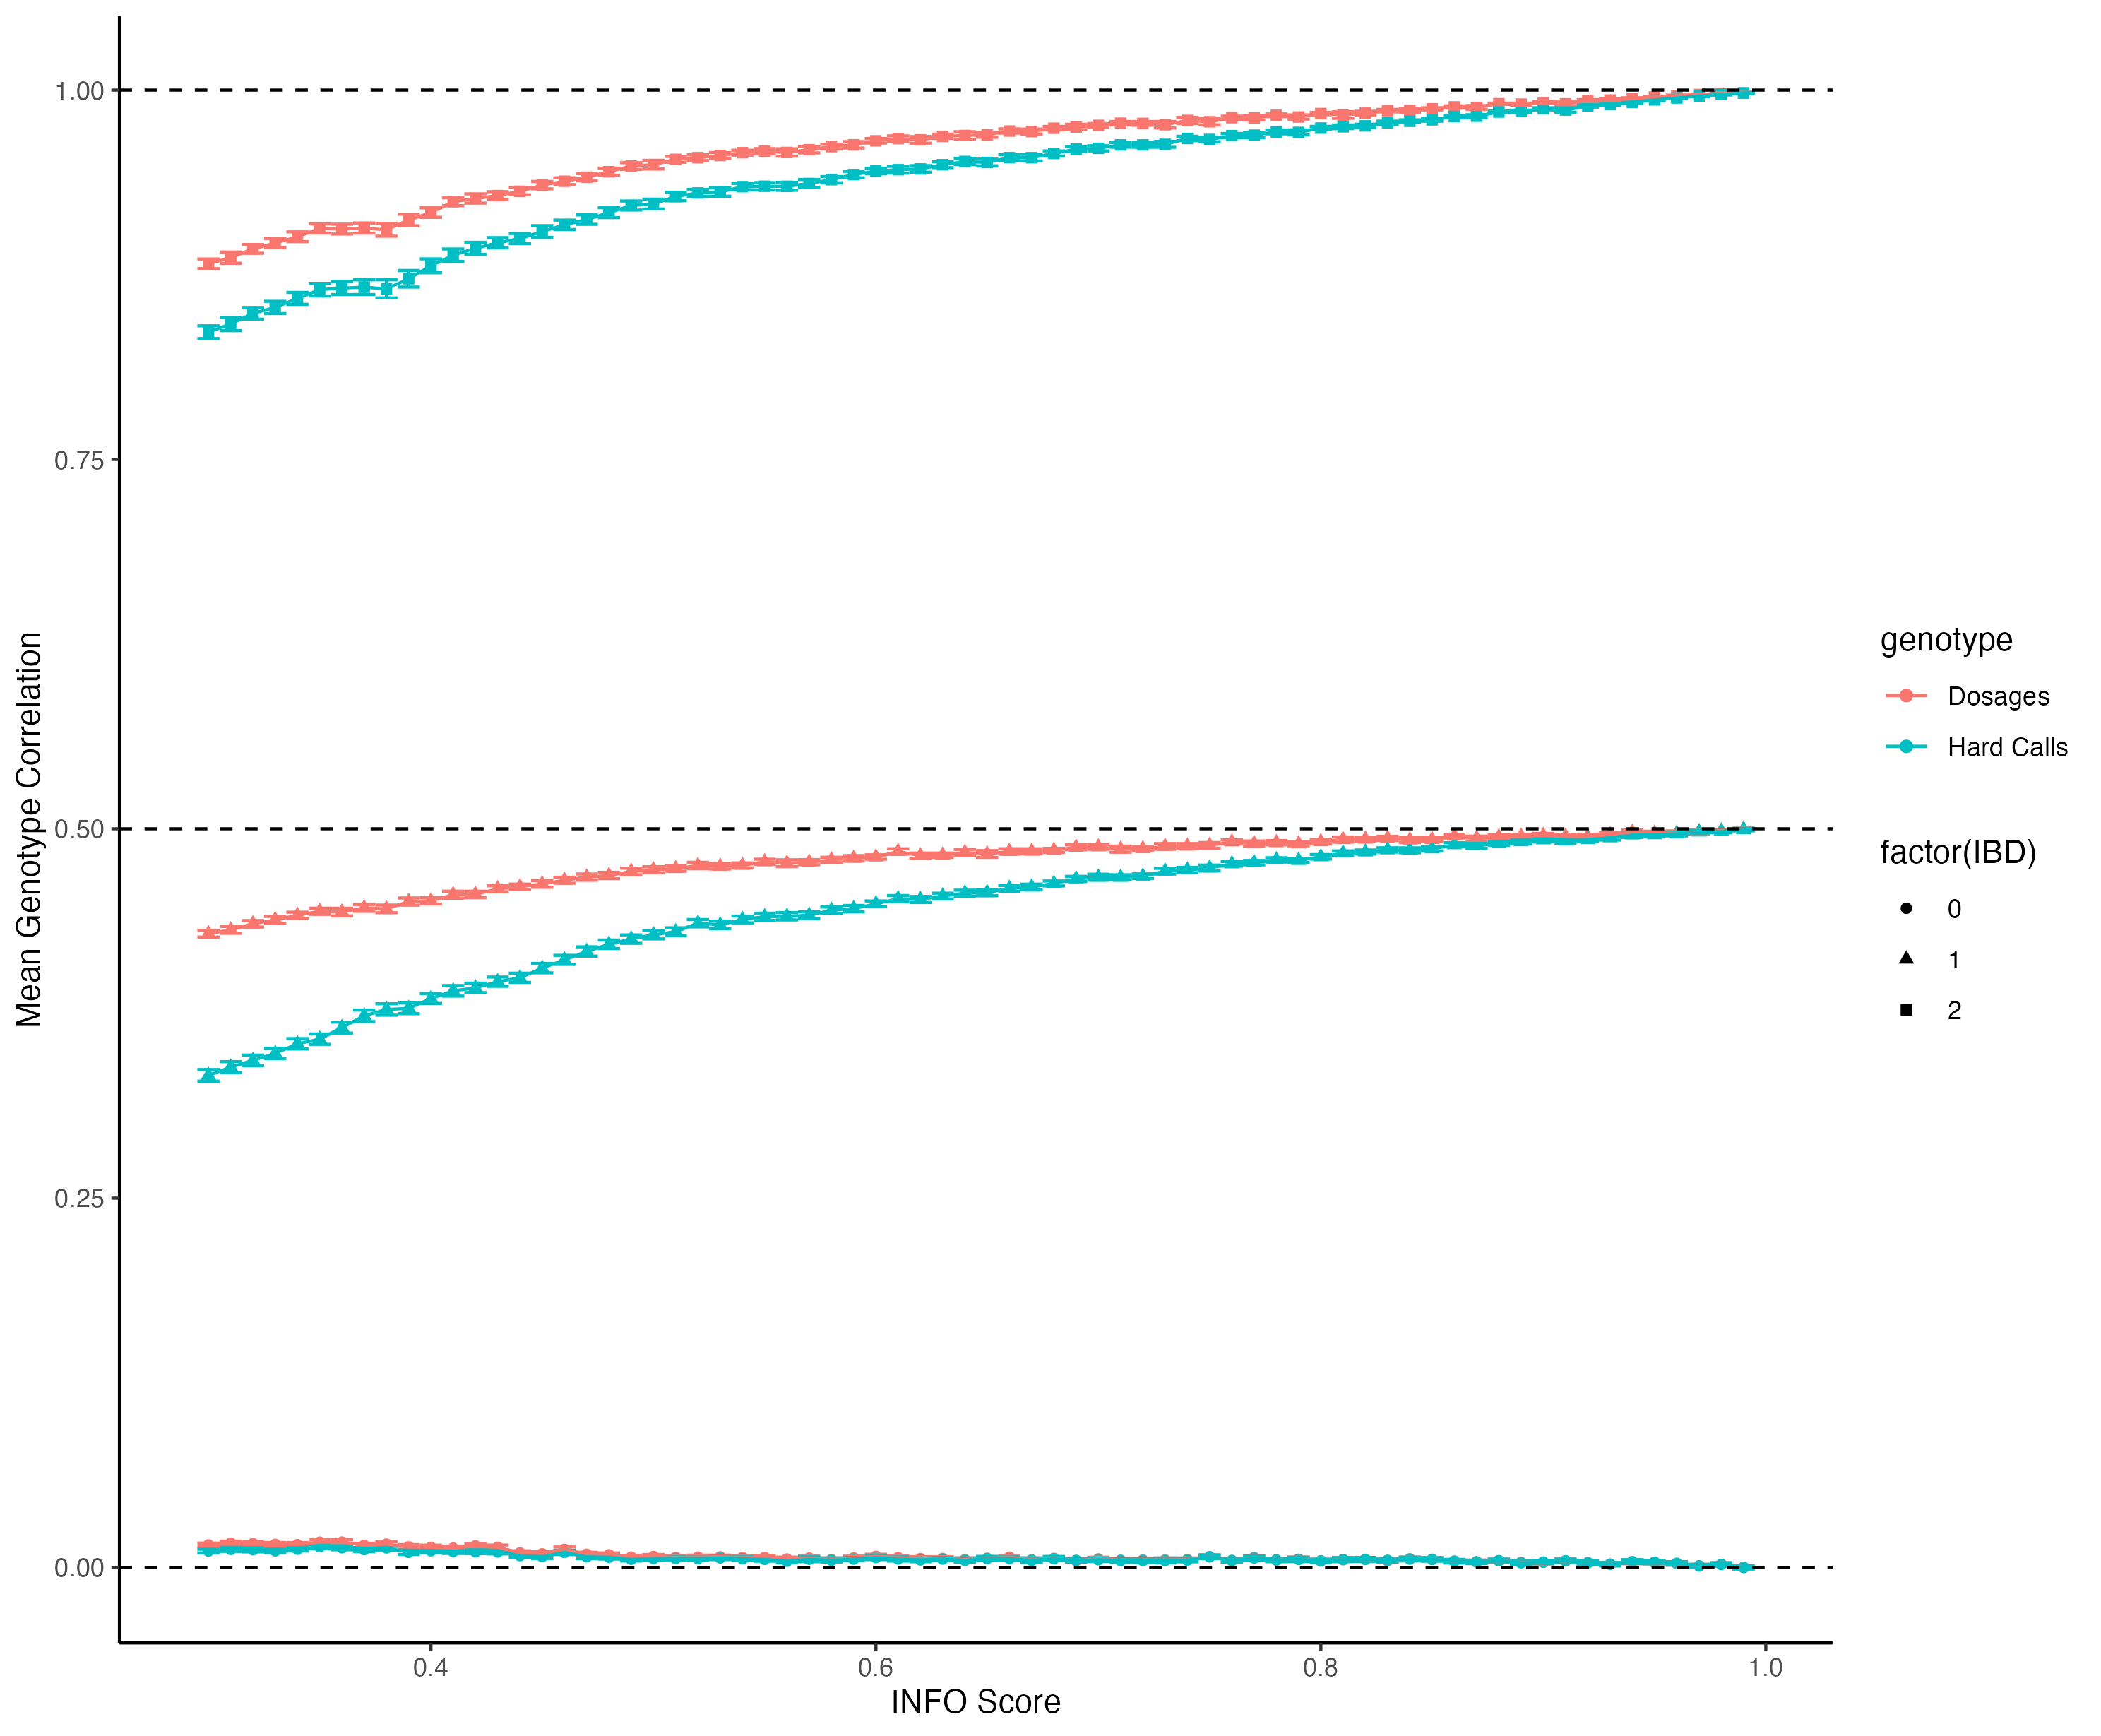
\includegraphics[width= .80\textwidth]{fig/mean_gt_by_ibd.png}
      \end{figure}
      % Briefly discuss the findings presented in this figure and their relevance.
\end{frame}

\begin{frame}{Next Steps}
      \begin{itemize}
            \item Using recently released WGS data from UKB. We are interesed to see what is the 
            the downstream effect of using low-quality imputed genotypes in GWAS analysis.
            \item We can do that by comparing the results of GWAS analysis using imputed genotypes and the WGS data.
\end{itemize}
\end{frame}

\begin{frame}{Next Steps}
    \begin{itemize}
      \item We still need imputation methods because it sill increase sample size. Like parental imputation of those in UKB data.
      \item Imputation methods don't take into account the relationships so for a pair of siblings, the imputaion is done independently.
      But in reality there are some information that can be used to improve the imputation quality from the other sibling in the pair.
      In other words the better imputation method should keep the correlation between the genotypes of the siblings.
      \item We are indterested in developing imputation methods that take into account the relationships between the individuals.
    \end{itemize}
\end{frame}

\begin{frame}[plain]
      \huge{Thank You!}
      % Conclude by thanking the audience and inviting any questions.
\end{frame}


\end{document}
